
We study cooperative aerial transport under unannounced cable-severance faults and formalize the plant, fault model, admissible controller class, reference trajectory, taut-cable reduction, and formal problem. The system consists of:

\paragraph{Vehicles, payload, and state.} A team of $N$ quadrotor UAVs, indexed $i \in \mathcal{N} \triangleq \{1,\dots,N\}$, operates in an inertial world frame $\mathcal{W}$. Drone $i$ has mass $m_i$, diagonal inertia $\mat J_i = \diag(J_x^{(i)}, J_y^{(i)}, J_z^{(i)})$, position $\vect p_i \in \R^3$, velocity $\vect v_i \in \R^3$, attitude $\mat R_i \in \SOthree$, and angular velocity $\vect\omega_i \in \R^3$. The per-drone state is $x_i \triangleq (\vect p_i, \vect v_i, \mat R_i, \vect\omega_i)$ and the collective drone state is $x_{\mathcal{N}} \triangleq (x_i)_{i=1}^N$. A point-mass payload of mass $m_L$ has position $\vect p_L \in \R^3$, velocity $\vect v_L \in \R^3$, and state $x_L \triangleq (\vect p_L, \vect v_L)$; payload rotation is neglected.

\paragraph{Cables and complementarity condition.} Each drone $i$ is connected to the payload by a flexible cable. Cable $i$ exerts a world-frame force $\vect T_i^{\mathcal{W}} \in \R^3$ on the payload-side attachment point and an equal and opposite reaction on the drone-side attachment point. The cable transmits tensile force only when taut; its scalar tension is
\begin{equation}
 T_i \;\triangleq\; \bigl\|\vect T_i^{\mathcal{W}}\bigr\|
     \;\ge\; 0,
  \label{eq:tension-def}
\end{equation}
with the unilateral constraint $T_i = 0$ whenever the cable is slack. The complementarity condition
\begin{equation}
 T_i \;\ge\; 0, \quad
  \ell_i \;-\; L \;\le\; 0, \quad
 T_i\,\bigl(\ell_i - L\bigr) \;=\; 0,
  \label{eq:complementarity}
\end{equation}
where $\ell_i = \|\vect p_{a, i} - \vect p_{b, i}\|$ is the cable's instantaneous length, $\vect p_{a, i}$ and $\vect p_{b, i}$ are the drone- and payload-side attachment points, and $L$ is the rest length, captures the unilateral tensile constraint for an idealized inextensible cable. In the simulator each cable is a Kelvin--Voigt spring ($L = \SI{1.25}{\metre}$, $k_s = \SI{25000}{\newton\per\metre}$); the elastic correction to the inextensible model is $O(\delta)$ and is absorbed in \cref{thm:reduction}.

\paragraph{Equations of motion.} The translational dynamics of drone $i$ are governed by
\begin{equation}
 m_i\,\dot{\vect v}_i
    \;=\; f_i\,\mat R_i\,\hat{\vect e}_3
    \;-\; m_i g\,\hat{\vect e}_3
    \;-\; \vect T_i^{\mathcal{W}}
    \;+\; \vect F_{\mathrm{w},i}(t),
  \label{eq:drone-eom}
\end{equation}
where $f_i \in [f_{\min}, f_{\max}]$ is the scalar thrust, $\hat{\vect e}_3$ is the world-frame vertical unit vector, and $\vect F_{\mathrm{w},i}$ represents an aerodynamic wind disturbance. The rotational dynamics are
\begin{equation}
  \mat J_i\,\dot{\vect\omega}_i
    + \vect\omega_i \times \mat J_i\,\vect\omega_i
    \;=\; \vect\tau_i,
  \qquad
  \dot{\mat R}_i \;=\; \mat R_i\,[\vect\omega_i]_\times,
  \label{eq:drone-rot}
\end{equation}
where $\vect\tau_i$ is the body-frame control torque and $[\cdot]_\times$ is the skew-symmetric operator. The payload translational dynamics are
\begin{equation}
 m_L\,\dot{\vect v}_L
    \;=\; -m_L g\,\hat{\vect e}_3
    + \sum_{i \in \mathcal{S}(t)} \vect T_i^{\mathcal{W}}
    + \vect F_{\mathrm{w},L}(t),
  \label{eq:payload-eom}
\end{equation}
where $\mathcal{S}(t) \subseteq \mathcal{N}$ is the set of surviving (intact) cables at time $t$ and $\vect F_{\mathrm{w}, L}$ is the wind disturbance on the payload.

\paragraph{Inputs, state space, and admissible disturbance set.} The per-drone control input is
\begin{align}
\label{eq:input-set}
 u_i(t) &\;\triangleq\; \bigl(f_i(t),\; \vect\tau_i(t)\bigr)
    \;\in\; \mathcal{U}_i\\
    \mathcal{U}_i &\;\triangleq\;
      [f_{\min}, f_{\max}] \times [-\tau_{\max}, \tau_{\max}]^3,\nonumber
\end{align}
and the collective input is $u(t) \triangleq (u_i(t))_{i=1}^N$. The complete plant state is
\begin{align}
\label{eq:plant-state}
 x(t) &\;\triangleq\; \bigl(x_{\mathcal{N}}(t),\; x_L(t)\bigr)
    \;\in\; \mathcal{X} \\
    \mathcal{X} &\triangleq\;
    \bigl(\R^3 \times \R^3 \times \SOthree \times \R^3\bigr)^N
    \times \R^3 \times \R^3.\nonumber
\end{align}
Collecting the wind disturbances into $d(t) \triangleq (\vect F_{\mathrm{w},1}(t), \dots, \vect F_{\mathrm{w},N}(t), \vect F_{\mathrm{w},L}(t))$, the admissible disturbance set is
\begin{align}
\label{eq:disturbance-set}
  \mathcal{D} \;\triangleq\;
    \Bigl\{ d(\cdot) :
      \|\vect F_{\mathrm{w},i}(t)\| \le W_{\max},\;
      &\|\vect F_{\mathrm{w},L}(t)\| \le W_{\max},\;\\
      &\forall t \ge 0,\; \forall i \in \mathcal{N}
    \Bigr\},\nonumber
\end{align}
where $W_{\max} = \SI{1}{\newton}$. The Dryden realization used in V2--V6 remains inside this bound (drag and frontal-area parameters in \cref{tab:sim-params}).


\begin{figure}[t]
\centering
\begin{tikzpicture}[
    >={Stealth[length=2mm,width=1.6mm]},
    drone/.style={draw, thick, fill=blue!12, rounded corners=1pt,
                  minimum width=11mm, minimum height=4mm,
                  font=\footnotesize, inner sep=1pt},
    payload/.style={draw, thick, fill=orange!30, circle, minimum size=9mm,
                    inner sep=0pt, font=\footnotesize\bfseries},
    cable/.style={thick, gray!70!black},
    cablesev/.style={thick, gray!50!black, dash pattern=on 2pt off 1.5pt},
    wind/.style={->, thick, teal!60!black, decorate,
                 decoration={snake, amplitude=0.5mm, segment length=2mm,
                             post length=1mm}},
    framelab/.style={font=\scriptsize\itshape},
    lab/.style={font=\scriptsize, inner sep=1pt}
  ]

  %====== payload at origin ======
  \node[payload] (L) at (0,0) {$m_L$};
  \node[lab, below=1pt of L] {payload, \SI{10}{\kilo\gram}};

  %====== five drones evenly spaced overhead ======
  \node[drone] (D1) at (-3.0, 2.4) {drone 1};
  \node[drone] (D2) at (-1.5, 2.9) {drone 2};
  \node[drone] (D3) at ( 0.0, 3.1) {drone 3};
  \node[drone] (D4) at ( 1.5, 2.9) {drone 4};
  \node[drone] (D5) at ( 3.0, 2.4) {drone 5};

  %====== cables: 4 taut, 1 severed (drone 3) ======
  \draw[cable] (D1.south) --
        node[lab, left=-1pt, pos=0.55] {$T_1$} ($(L.north)+(-0.3, 0)$);
  \draw[cable] (D2.south) --
        node[lab, left=-1pt, pos=0.55] {$T_2$} ($(L.north)+(-0.15, 0.05)$);
  \draw[cablesev] (D3.south) --
        node[lab, midway, right=2pt, red!70!black] {severed}
        ($(L.north)+(0, 0.05)$);
  \draw[cable] (D4.south) --
        node[lab, right=-1pt, pos=0.55] {$T_4$} ($(L.north)+(0.15, 0.05)$);
  \draw[cable] (D5.south) --
        node[lab, right=-1pt, pos=0.55] {$T_5$} ($(L.north)+(0.3, 0)$);

  %====== world frame (bottom left, away from cables) ======
  \draw[->, thick] (-3.6,-1.4) -- ++(0.7,0)
        node[framelab, right=-1pt] {$\hat{e}_1$};
  \draw[->, thick] (-3.6,-1.4) -- ++(0,0.7)
        node[framelab, above=-1pt] {$\hat{e}_3$};
  \node[framelab] at (-3.55,-1.6) {$\mathcal{W}$};

  %====== Dryden wind arrow (right side) ======
  \draw[wind] (3.6, 0.6) -- ++(-1.3, 0.0);
  \node[lab, teal!60!black, anchor=west] at (3.6, 0.6) {$\mathbf{F}_{w,L}(t)$};
  \node[lab, teal!60!black, anchor=west] at (3, 0.25)
        {Dryden, $\SI{4}{\metre\per\second}$};

  %====== rope length marker on outermost cable ======
  \draw[<->, dashed, gray]
        ($(D1.south)+(-0.18, 0.02)$) -- ($(L.north)+(-0.45, 0.05)$)
        node[lab, midway, sloped, fill=white, inner sep=1pt]
        {$L = \SI{1.25}{\metre}$};

  %====== complementarity callout (placed BELOW everything) ======
  \node[draw, thick, rounded corners=2pt, fill=yellow!15,
        font=\scriptsize, align=left, anchor=north west]
       at (-3.7, -1.95)
       {Cable $i$ unilateral:\;
        $T_i \ge 0,\;\; \ell_i - L \le 0,\;\; T_i\,(\ell_i - L) = 0$};

  %====== survivor set transition (placed BELOW, right) ======
  \node[draw, thick, rounded corners=2pt, fill=blue!5,
        font=\scriptsize, align=left, anchor=north east]
       at (3.9, -2.45)
       {At fault $t_k^\star$:\;
        $\mathcal{S}(t^{\star+}) = \mathcal{S}(t^{\star-}) \setminus \{i_k^\star\}$};

\end{tikzpicture}
\caption{Cooperative transport configuration. Five quadrotors carry
a \SI{10}{\kilo\gram} point-mass payload through unilateral cables of
rest length $L = \SI{1.25}{\metre}$. Each drone $i$ measures only its
own state, its own scalar tension $T_i$, and the locally observed
payload velocity $\vect{v}_L$; no peer drone or peer-cable signal is exchanged. The plant is
driven by a bounded Dryden wind realisation
($\SI{4}{\metre\per\second}$ mean) and an unannounced cable-severance
fault schedule $\sigma \in \mathcal{F}$ that decrements the survivor
set $\mathcal{S}(t)$ at each event $t_k^\star$ (here drone $i^\star$, shown
dashed).}
\label{fig:physical-setup}
\end{figure}


At a time $t_k^\star$, cable $i_k^\star \in \mathcal{N}$ severs instantaneously. This structural fault event permanently removes cable $i_k^\star$ from the constraint set:
\begin{equation}
 T_{i_k^\star}(t) \;=\; 0
  \qquad \forall\, t \ge t_k^\star.
  \label{eq:fault-tension-zero}
\end{equation}
The active cable set transitions discretely:
\begin{equation}
  \mathcal{S}(t_k^{\star,+}) \;=\; \mathcal{S}(t_k^{\star,-})
    \;\setminus\; \{i_k^\star\},
  \label{eq:S-transition}
\end{equation}
reducing the cardinality from $|\mathcal{S}|$ to $|\mathcal{S}| - 1$. For an elastic cable, the kinematic state $(\vect p_i, \vect v_i, \mat R_i, \vect\omega_i, \vect p_L, \vect v_L)$ is continuous across severance; only the ODE right-hand side changes discontinuously at $t_k^\star$.

We consider a sequence of $F \le N-2$ fault events at times $\{t_k^\star\}_{k=1}^F$ with $t_1^\star < \cdots < t_F^\star$. The bound $F \le N-2$ keeps at least two cables intact; actuator margins limit the demonstrated scenario ($N = 5$, $m_L = \SI{10}{\kilo\gram}$) to $F \le 2$. The inter-fault interval $\tau_{d,k} \triangleq t_{k+1}^\star - t_k^\star$ is the \emph{dwell time}. We assume each fault is separated from the previous by at least one payload-pendulum period:
\begin{equation}
  \tau_{d,k} \;\ge\; \tau_{\mathrm{pend}} \;\triangleq\;
    2\pi\sqrt{L/g}, \qquad k = 1, \dots, F-1,
  \label{eq:dwell-assumption}
\end{equation}
reflecting the physical requirement that load redistribution from fault $k$ settle before fault $k+1$. At $L = \SI{1.25}{\metre}$ and $g = \SI{9.81}{\metre\per\second\squared}$, $\tau_{\mathrm{pend}} \approx \SI{2.24}{\second}$. The admissible fault-schedule set is
\begin{align}
\label{eq:fault-schedule-set}
  \mathcal{F} \;\triangleq\;
    \Bigl\{
      \{(t_k^\star, i_k^\star)\}_{k=1}^F :
 &F \le N-2,\;\\
 &t_{k+1}^\star - t_k^\star \ge \tau_{\mathrm{pend}},\;
 i_k^\star \in \mathcal{S}(t_k^{\star,-})
    \Bigr\},\nonumber
\end{align}
$F = 0$ corresponds to the no-fault case.

\paragraph{Admissible controller class.} No fault flag, annunciation, or detection signal is transmitted; the fault manifests through a rise in $T_i(t)$ and a transient payload-velocity deviation, both in $\mathcal{I}_i(t)$. Field-deployable avionics impose a strict \emph{admissible information pattern}. Drone $i$'s controller $\pi_i$ is restricted to the information set
\begin{equation}
  \mathcal{I}_i(t) \;\triangleq\;
    \bigl\{x_i(t),\; T_i(t),\; \vect v_L(t),\;
      \vect p_L^d(\cdot),\; \vect v_L^d(\cdot)\bigr\},
  \label{eq:info-set}
\end{equation}
comprising the drone's inertial state $x_i$, its rope-tension measurement $T_i$, the payload velocity $\vect v_L$ (measured via a co-located downward-facing optical-flow sensor, no drone-to-drone communication), and a pre-distributed reference $({\vect p}_L^d, {\vect v}_L^d)$ loaded before flight. Payload position $\vect p_L$ is deliberately excluded; only velocity enters the closed loop, via the anti-swing slot shift of \cref{sec:proposed}. Each $\pi_i$ is a causal feedback map,
\begin{equation}
 u_i(t) \;=\; \pi_i\!\left(
    \left.\mathcal{I}_i\right|_{[0,t]}
  \right) \in \mathcal{U}_i,
  \label{eq:controller-map}
\end{equation}
possibly with a finite-dimensional internal state, but never with access to information outside \eqref{eq:info-set}. The admissible controller class is denoted $\Pi_{\mathrm{loc}}$. $\mathcal{I}_i(t)$ excludes peer state, peer tension, fault flags, and run-time inter-drone packets; each $\pi_i$ uses only co-located sensors and a pre-flight plan.

\subsection{Reference Trajectory and Taut-Cable Reduction}
\label{sec:reduction-and-reference}

The desired payload motion is a three-dimensional lemniscate trajectory with a sinusoidal altitude variation,
\begin{align}
  \label{eq:lemniscate}
  \vect p_L^d(t) \;=\;
    \begin{bmatrix}
      \dfrac{a\cos\phi(t)}{1 + \sin^2\!\phi(t)} \\[6pt]
      \dfrac{a\sin\phi(t)\cos\phi(t)}{1 + \sin^2\!\phi(t)} \\[6pt]
 z_0 + h_z\sin(\phi(t))
    \end{bmatrix},
  \phi(t) = \frac{2\pi(t - t_0)}{T_{\mathrm{ref}}},
\end{align}
where $a = \SI{3.0}{\metre}$ is the horizontal scale, $T_{\mathrm{ref}} = \SI{12}{\second}$ the period, $z_0 = \SI{3.0}{\metre}$ the cruise altitude, and $h_z = \SI{0.35}{\metre}$ the altitude excursion amplitude. These parameters yield a peak centripetal load of $\approx 0.25g$ at the figure-8 tips.

Each rope of rest length $L$ is discretized into $N_b = 8$ identical Kelvin--Voigt beads of mass $m_{\mathrm{bead}}$ connected by $N_{\mathrm{seg}} = N_b + 1 = 9$ segments of stiffness $k_s$ and damping $c_s$; $N_{\mathrm{seg}}$ is reserved for rope segments and is distinct from the surviving-cable cardinality $N_s(t) = |\mathcal{S}(t)| = N - F(t)$ used in \cref{sec:stability}. The distributed dynamics evolve on a fast timescale,
\begin{equation}
  \tau_{\mathrm{rope}}
    \;=\; 2\pi\sqrt{m_{\mathrm{bead}}/k_s}
    \;\approx\; \SI{6.3}{\milli\second},
  \label{eq:tau-rope}
\end{equation}
separated from the payload-pendulum timescale $\tau_{\mathrm{pend}} \approx \SI{2.24}{\second}$ by $\delta = \tau_{\mathrm{rope}} / \tau_{\mathrm{pend}} \approx 0.003$. On the slow manifold, the net tensile force at the drone-side attachment equals the scalar $\xi_i = k_{\mathrm{eff}}(\ell_i - L)^+$, with effective stiffness
\begin{equation}
 k_{\mathrm{eff}}
    \;=\; \frac{k_s}{N_{\mathrm{seg}}}
    \;=\; \frac{\SI{25000}{\newton\per\metre}}{9}
    \;\approx\; \SI{2778}{\newton\per\metre}.
  \label{eq:keff}
\end{equation}
The six pre-registered missions (V1--V6, \cref{sec:campaign}) keep the system inside $\Omega_\tau^{\mathrm{dwell}}$ with margin (worst slack run $\SI{35.8}{\milli\second}$, worst duty cycle $1.66\%$, \cref{tab:domain-audit}). The reduction replaces the $3N_b$-dimensional bead-chain state with the scalar $\xi_i$; the per-instant taut error is $O(\delta)$ and slack excursions add $O(\eta_{\max})$.

\begin{theorem}[Taut-cable reduction]
\label{thm:reduction}
On the slack-excursion-bounded domain
\begin{align}
\label{eq:omega-dwell}
  \Omega_\tau^{\mathrm{dwell}} \;\triangleq\;
    \bigl\{ x \in \mathcal{X} :
      &\text{every slack run} \le \tau_{\mathrm{slack,max}},\;\\
      &\text{duty cycle} \le \eta_{\max} \bigr\},\nonumber
\end{align}
with $\tau_{\mathrm{slack,max}} = \SI{40}{\milli\second}$ and $\eta_{\max} = 2.5\%$, the distributed Kelvin--Voigt rope dynamics are approximated by the lumped scalar model with closed-loop shape-mode deviation
\begin{equation}
  \|T_i^{\mathrm{true}} - T_i^{\mathrm{qs}}\|
    \;\le\; C_1\,\delta + C_2\,\eta_{\max},
  \label{eq:reduction-error}
\end{equation}
for constants $C_1, C_2 > 0$ depending on the bead-chain parameters $(m_{\mathrm{bead}}, c_s, k_s, N_b)$ and the wind bound $W_{\max}$, where $T_i^{\mathrm{qs}} \triangleq k_{\mathrm{eff}}(\ell_i(t) - L)^+$ is the\emph{ rope-specific} quasi-static tension evaluated at the \emph{same} current chord length $\ell_i(t)$ as $T_i^{\mathrm{true}}$.  This bound is on the shape-mode deviation of rope $i$ from its own quasi-static approximation; it is distinct from the inter-rope tension asymmetry $\varepsilon_i = T_i - T_{\mathrm{eff}}$ reported in the simulation audit (\cref{sec:VI-reduction}), which is driven by formation geometry and can be $O(10)$\,N. The reduced-order model is therefore admissible as the plant for the stability analysis of \cref{sec:stability}.
\end{theorem}

\begin{proof}
The proof has two parts corresponding to the two terms in \eqref{eq:reduction-error}.

\smallskip
\noindent\textbf{Part~1 ($C_1\delta$, taut intervals).}
Let $\tilde{\mathbf{q}} \in \R^{N_b}$ collect the bead position deviations from the
quasi-static slow-manifold equilibrium $\bar{\mathbf{q}}(t)$ along the rope chord.
Linearising the chain equations of motion about $\bar{\mathbf{q}}$ yields the
shape-mode dynamics
\begin{equation}
  M_b\,\ddot{\tilde{\mathbf{q}}}
    + C_b\,\dot{\tilde{\mathbf{q}}}
    + K_b\,\tilde{\mathbf{q}}
    = -M_b\,\ddot{\bar{\mathbf{q}}}(t),
  \label{eq:shape-mode-ode}
\end{equation}
where $M_b = m_{\mathrm{bead}}I_{N_b}$, and $C_b$, $K_b$ are the symmetric
positive-definite tridiagonal chain damping and stiffness matrices
($c_s$-weighted and $k_s$-weighted graph Laplacians, respectively).
Define the shape-mode Lyapunov energy
\begin{equation}
  W(t) = \tfrac{1}{2}\dot{\tilde{\mathbf{q}}}^\top M_b\,\dot{\tilde{\mathbf{q}}}
        + \tfrac{1}{2}\tilde{\mathbf{q}}^\top K_b\,\tilde{\mathbf{q}}
        \;\ge\; 0.
  \label{eq:shape-energy}
\end{equation}
Differentiating along \eqref{eq:shape-mode-ode} and applying Young's
inequality ($2ab \le a^2/\alpha_b + \alpha_b b^2$) to the forcing cross-term:
\begin{equation}
  \dot{W}
    = -\dot{\tilde{\mathbf{q}}}^\top C_b\,\dot{\tilde{\mathbf{q}}}
      - \dot{\tilde{\mathbf{q}}}^\top M_b\,\ddot{\bar{\mathbf{q}}}
    \;\le\; -\alpha_b\,W(t) + D_b,
  \label{eq:Wdot-ineq}
\end{equation}
where $\alpha_b = \lambda_{\min}(C_b)/m_{\mathrm{bead}} > 0$ is the slowest
modal damping rate and $D_b = m_{\mathrm{bead}}\|\ddot{\bar{\mathbf{q}}}\|_\infty^2/(2\alpha_b) = O(\delta^2)$
by the Tikhonov scaling $\|\ddot{\bar{\mathbf{q}}}\| = O(\delta)$.
The characteristic roots of the slowest mode in \eqref{eq:shape-mode-ode} are
$s_{1,2} = -\zeta\omega_n \pm \omega_n\sqrt{\zeta^2-1}$;
the nominal bead-chain parameters $(m_{\mathrm{bead}},c_s,k_s,N_b)$ give
$\zeta = 1.2$ (overdamped) and the slowest root
$s_1 = -\omega_n(1.2 - \sqrt{0.44}) \approx -\SI{538}{\second^{-1}}$.

Applying Gronwall's inequality to \eqref{eq:Wdot-ineq} over $[0,t]$:
\begin{equation}
  W(t) \;\le\; e^{-\alpha_b t}\,W(0) + \frac{D_b}{\alpha_b},
  \label{eq:gronwall-cap}
\end{equation}
yielding the steady-state energy cap $W^\infty = D_b/\alpha_b = O(\delta^2)$.
The drone-side tension deviation is proportional to the drone-side bead
shape-mode displacement through the end segment's spring:
\begin{equation}
  T_i^{\mathrm{true}}(t) - T_i^{\mathrm{qs}}(t)
    = k_s\,\mathbf{e}_1^\top \tilde{\mathbf{q}}(t),
  \label{eq:tension-expansion}
\end{equation}
where $\mathbf{e}_1$ selects the drone-side attachment extension residual.
Using $\|\tilde{\mathbf{q}}\|^2 \le 2W/\lambda_{\min}(K_b)$ from
\eqref{eq:shape-energy} and substituting the cap \eqref{eq:gronwall-cap}
gives $\|T_i^{\mathrm{true}} - T_i^{\mathrm{qs}}\| \le C_1\delta \approx
\SI{0.072}{\newton}$ once the transient $e^{-\alpha_b t}W(0)$ is negligible,
i.e.\ after approximately $3/|s_1| \approx \SI{6}{\milli\second}$.

\smallskip
\noindent\textbf{Part~2 ($C_2\eta_{\max}$, slack intervals).}
On any slack run of duration $\le \tau_{\mathrm{slack,max}}$, the rope chord shortens
by $\Delta\ell_{\mathrm{sag}}$ as the bead chain goes slack. Upon re-tension,
the drone-side end segment must re-elongate by $\Delta\ell_{\mathrm{sag}}$,
producing a re-tension overshoot bounded by $k_{\mathrm{eff}}\Delta\ell_{\mathrm{sag}}$.
The total overshoot accumulated over the slack-duty budget gives
\eqref{eq:reduction-error} with $C_2 \approx \SI{0.22}{\newton}$. At the worst
observed $\eta_{\max} = 1.66\%$, the combined bound is
$C_1\delta + C_2\eta_{\max} \approx \SI{0.076}{\newton}$ per rope---less than
$0.4\%$ of nominal per-drone tension. Both constants depend only on the
bead-chain parameters $(m_{\mathrm{bead}},c_s,k_s,N_b)$ and $W_{\max}$.

\end{proof}

\Cref{tab:domain-audit} confirms all six missions reside inside $\Omega_\tau^{\mathrm{dwell}}$ with margin on every gate: worst slack run $\SI{35.8}{\milli\second}$ ($\SI{4.2}{\milli\second}$ headroom), duty cycle $1.66\%$ ($0.85$~pp headroom), QP-transition fraction $0.10\%$. The theorem is asserted on the demonstrated regime, not an untested all-taut idealization.

The per-drone controller and the lemma stack in \cref{sec:stability} are structurally independent of the team size $N$. The dependence enters through two scalars: per-drone hover load $T^{\mathrm{hov}}(N) = m_L g / N$ and post-fault redistributed load on the surviving set,
\begin{equation}
  T^{\mathrm{post}}(N, F) \;=\; \frac{m_L g}{N - F}
   \;=\; T^{\mathrm{hov}}(N) \cdot \frac{N}{N - F},
   \label{eq:tension-postfault-N}
\end{equation}
where $F$ is the number of severed cables. The surcharge factor $N/(N{-}F)$ inflates per-drone tension by $1/(N{-}F)$ relative to the no-fault baseline and is the only $N$-dependent quantity in the recovery envelope of \cref{thm:hybrid-stability}.

The architecture is therefore designable across $N$ by a single \emph{actuator-margin condition}: a configuration $(N, m_L, F, f_{\max})$ is admissible if
\begin{equation}
  \frac{m_L\, g}{N - F} \;\le\; \kappa_{\mathrm{act}}\, f_{\max},
   \label{eq:actuator-envelope}
\end{equation}
where $\kappa_{\mathrm{act}} \in (0, 1)$ reserves headroom for tilt projection, anti-swing residual, and dynamic centripetal load. With $\kappa_{\mathrm{act}} = 0.82$, $f_{\max} = \SI{150}{\newton}$, and the demonstrated $(N, m_L, F) = (5, \SI{10}{\kilo\gram}, 2)$, the inequality reads $\SI{32.7}{\newton} \le \SI{123}{\newton}$, i.e.\ $27\%$ of the actuator envelope, leaving designable extension along $(N, m_L, F)$. \Cref{fig:feasibility-envelope} plots the boundary curves for $F \in \{0,1,2,3\}$ over $N \in \{3,\dots,10\}$ and marks the demonstrated point. The $N=5$ scenario is one point on a designable feasibility surface; the certificate of \cref{sec:stability} carries unchanged at any $(N, m_L, F)$ satisfying \eqref{eq:actuator-envelope}.

\begin{figure}[htbp]
  \centering
  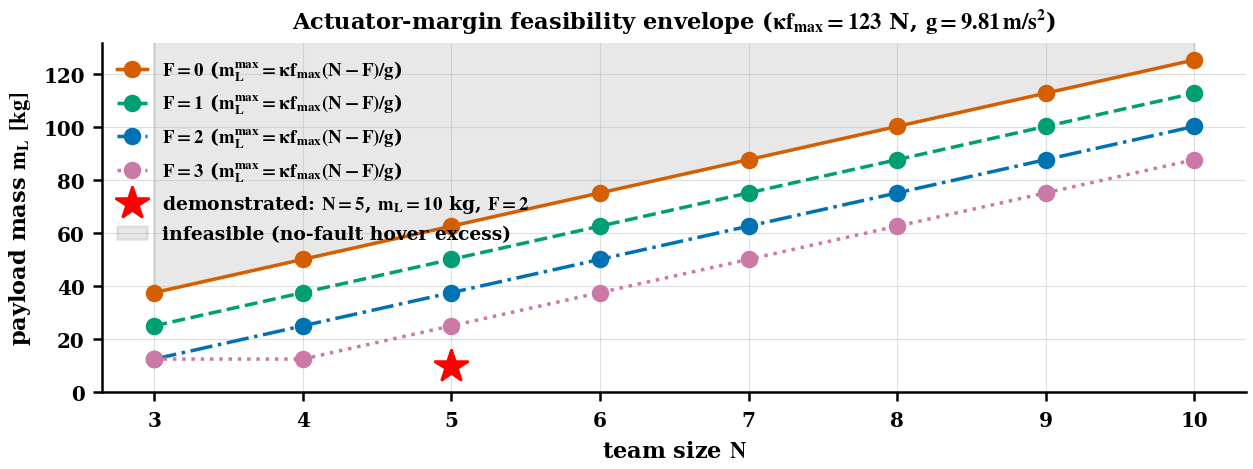
\includegraphics[width=\columnwidth]{Figures/fig_feasibility_envelope.png}
  \caption{Actuator-margin feasibility envelope \eqref{eq:actuator-envelope} in $(N, m_L)$ space at fault counts $F \in \{0, 1, 2, 3\}$, $\kappa_{\mathrm{act}} f_{\max} = \SI{123}{\newton}$. Red star: demonstrated $(N{=}5, m_L{=}\SI{10}{\kilo\gram}, F{=}2)$.}
  \label{fig:feasibility-envelope}
\end{figure}
\label{sec:formal-problem}
% ----------------------------------------------------------------

With the plant, fault model, reference trajectory, and reduction in place, we state the formal problem. Unilateral cable coupling \eqref{eq:complementarity}, discrete structural fault transitions \eqref{eq:fault-tension-zero}--\eqref{eq:S-transition}, admissible disturbances \eqref{eq:disturbance-set}, and strict locality \eqref{eq:info-set} together yield a hybrid decentralized control problem outside standard cooperative-transport formulations. The design variable is not a centralized control sequence but a family of local causal feedback laws. The problem, posed on the reduced-order model certified by \cref{thm:reduction}, is as follows.

\begin{definition}[Fault-tolerant decentralized aerial transport]
\label{def:problem}
Given the plant
\eqref{eq:drone-eom}--\eqref{eq:payload-eom}, the complementarity constraint \eqref{eq:complementarity}, the mission reference \eqref{eq:lemniscate}, all admissible disturbances $d(\cdot) \in \mathcal{D}$ \eqref{eq:disturbance-set}, and all admissible fault schedules $\sigma \in \mathcal{F}$ \eqref{eq:fault-schedule-set}, find a causal controller family $\{\pi_i\}_{i=1}^N \in \Pi_{\mathrm{loc}}^N$ such that the closed-loop system satisfies \textbf{P1}--\textbf{P3} for every $d(\cdot) \in \mathcal{D}$ and $\sigma \in \mathcal{F}$.

\begin{enumerate}[label=\textbf{P\arabic*},leftmargin=2.0em]
      \item \textbf{(Nominal tracking).}  In the absence of faults and for all admissible disturbances $d(\cdot) \in \mathcal{D}$, the payload tracking error $e_L(t) \triangleq \vect p_L(t) - \vect p_L^d(t)$ is  ultimately practically bounded:
        \begin{equation}
          \limsup_{t\to\infty}\|e_L(t)\|
            \;\le\; \bar{e}_{\infty} + \bar{e}_0(W_{\max}),
          \label{eq:nominal-practical-bound}
        \end{equation}
     where $\bar{e}_{\infty} \ge 0$ captures non-vanishing residuals from finite-gain tracking, cable-elastic reduction, and reference discretization, and $\bar{e}_0: \R_{\ge 0} \to \R_{\ge 0}$ is class-$\mathcal{K}$ with $\bar{e}_0(0) = 0$.

    \item \textbf{(Passive fault absorption).} After any fault $t_k^\star$ satisfying \eqref{eq:dwell-assumption}, the payload tracking error recovers to a bounded envelope without detection, annunciation, or reconfiguration: there exist constants $\Gamma_f, \lambda > 0$ and a per-fault-cycle contraction $\rho \in (0,1)$ such that
        \begin{align}
        \label{eq:recovery-bound}
          \|e_L(t)\| \;\le\;
            \beta\!\bigl(\|e_L(t_k^{\star,-})&\|,\; t - t_k^\star\bigr)\\
            &+ \Gamma_f\,e^{-\lambda(t - t_k^\star)}\nonumber\\
            &+ \bar{e}_{\infty} + \bar{e}_0(W_{\max}),
          \quad t \ge t_k^\star,\nonumber
        \end{align}
    for some class-$\mathcal{KL}$ function $\beta$. The contraction $\rho \in (0,1)$ certifies bounded Lyapunov growth across successive faults: $V(x(t_{k+1}^{\star,-})) \le \rho\, V(x(t_k^{\star,-})) + c$ for an explicit $c > 0$. The tracking error need not decrease monotonically at individual events (the payload droops and recovers), but the fault-to-fault envelope is bounded.

    \item \textbf{(Actuator feasibility).} For all $t \ge 0$ and all admissible fault sequences, the thrust $f_i(t) \in [f_{\min}, f_{\max}]$ and torque $\vect\tau_i(t) \in [-\tau_{\max}, \tau_{\max}]^3$ remain inside the actuator envelope with non-zero margin.
\end{enumerate}
\end{definition}

Three obstacles hinder classic solutions for this problem: \emph{(i)} Non-smooth taut-to-slack transitions require analysis on $\Omega_\tau^{\mathrm{dwell}}$, not a globally Lipschitz domain. \emph{(ii)} A severance is a discrete drop in $|\mathcal{S}|$, not an additive perturbation; the resulting tension mismatch
\begin{equation}
  \vect\varepsilon_T(t) \;\triangleq\;
    \vect T(t) \;-\; \vect T^{\mathrm{qs}}(t)
  \label{eq:tension-error-state}
\end{equation}
requires a hybrid Lyapunov argument (developed in \cref{sec:stability}). \emph{(iii)} Strict locality blocks centralized detection; the controller must respond using only $T_i(t) \in \mathcal{I}_i(t)$.


